\documentclass[tikz,border=2pt]{standalone}
\usepackage{amsmath,amssymb}
\usepackage{pgfplots}
\pgfplotsset{compat=1.18}

\begin{document}
% g(x, y) = xy on the unit square with uniform density 1: level curves xy = c. The expectation
% E[XY] is the density-weighted average of g over the square, 1/4.
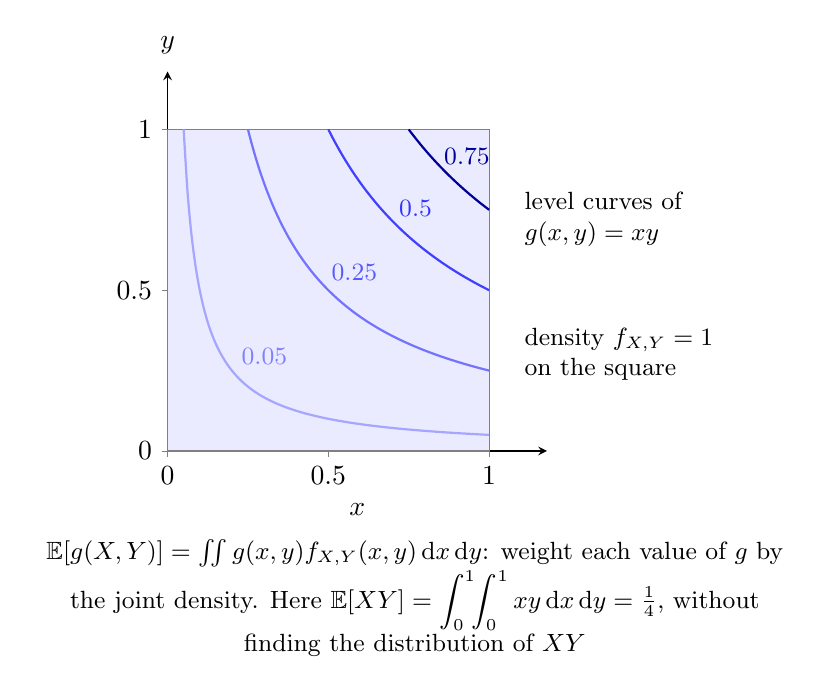
\begin{tikzpicture}
	\begin{axis}[
		axis lines=left, xmin=0, xmax=1.18, ymin=0, ymax=1.18,
		xtick={0,0.5,1}, ytick={0,0.5,1},
		xlabel={$x$}, ylabel={$y$}, ylabel style={rotate=-90, anchor=south, at={(axis description cs:0,1.02)}},
		samples=80, smooth, width=6.4cm, height=6.4cm, clip=false
		]
		\fill[blue!8] (axis cs:0,0) rectangle (axis cs:1,1);
		\draw[gray] (axis cs:0,0) rectangle (axis cs:1,1);
		\addplot[blue!35, thick, domain=0.05:1] {0.05/x};
		\addplot[blue!55, thick, domain=0.25:1] {0.25/x};
		\addplot[blue!75, thick, domain=0.5:1] {0.5/x};
		\addplot[blue!60!black, thick, domain=0.75:1] {0.75/x};
		\node[blue!50, font=\small, anchor=south west] at (axis cs:0.2,0.24) {$0.05$};
		\node[blue!65, font=\small, anchor=south west] at (axis cs:0.48,0.5) {$0.25$};
		\node[blue!80, font=\small, anchor=south west] at (axis cs:0.69,0.7) {$0.5$};
		\node[blue!60!black, font=\small, anchor=south west] at (axis cs:0.83,0.86) {$0.75$};
		\node[anchor=west, font=\small, align=left] at (axis cs:1.08,0.72) {level curves of\\ $g(x,y)=xy$};
		\node[anchor=west, font=\small, align=left] at (axis cs:1.08,0.3) {density $f_{X,Y}=1$\\ on the square};
	\end{axis}
	\node[anchor=north, font=\small, align=flush center, text width=9.6cm] at ([yshift=-2pt]current axis.outer south) {$\mathbb{E}[g(X,Y)]=\iint g(x,y)f_{X,Y}(x,y)\,\mathrm{d}x\,\mathrm{d}y$: weight each value of $g$ by the joint density. Here $\mathbb{E}[XY]=\displaystyle\int_0^1\!\!\int_0^1xy\,\mathrm{d}x\,\mathrm{d}y=\tfrac14$, without finding the distribution of $XY$};
\end{tikzpicture}
\end{document}
